\newpage
\section{Evalutaion einer symmetrischen Antenne}
Das Abstrahlverhalten von Loop und Dipol Antennen ist im Fernfeld gleich. Im Fernfeld steht das E und das H Feld senkrech aufeinander. Senkrecht zu E und H Feld zeigt der Ausbreitungsvektor. Die elektrische und magnetische Feldkomponente sind in Phase, daher wird im Fernfeld Wirkleistung in transversale Raumrichtung übertragen. Das elektrische und magnetische Feld hat nur Komponenten in der Ebene senkrecht zur Ausbreitungsrichtung. Man Spricht von einer ebenen Welle die vom E und H Vektor aufgespannt wird und sich in Transversalerrichtung fortbewegt, bis  die gemammte Energie absorbiert ist. Die Amplituden der E und H Vektoren nemhen mit steigendem Abstand r um den Faktor $1/r$ ab. Der Zusammenhang wischen E und H Feld ist durch die intrinsische Wellenimpedanz gegeben. Die Gleichung \ref{eq:WellenImpedanzZ0} zeigt, den Wellenwiderstand im Vakuum.

\begin{equation}\label{eq:WellenImpedanzZ0}
Z_{0}=\dfrac{E}{H}=\sqrt{\dfrac{\mu}{\epsilon}}=377\Omega
\end{equation}



Die Ausrichtung des E Feld ist bei Loop und Dipol Antennen um 90 Grad verschoben. 
Im Nahfeld sind die Induktiven Anteile des elektromagnetischen Wechselfeld bei der Loop Antenne dominant. 
Im Gegenzug ist das Nahfeld der Dipol Antenne mehr kapazitiv.
Mann nennt die Dipolantenne deshalb E Feld Antenne und die Loop Antenne wird oft H Feld Antenne genannt.
Das Abstrahlverhalten ist in den Kapitelen \ref{sec:DipolAntenne} und \ref{sec:LoopAntenneTheorie} aufgezeigt. Die Abbildung \ref{fig:FerdVektorEinheistsvektor} zeigt einen Pointingvektor im  Kugelkoordinaten- und im Kartesischen Koordinatensystem am Ende des Pointingvektor r ist sind die Einheisvektoren mit den daszugehörenden E- und H Feldvektoren.\\

%%%%%%%%%%%%%%%%%%%%%%%%%%%%%%%%%%%
\begin{figure}[h]
\begin{center}
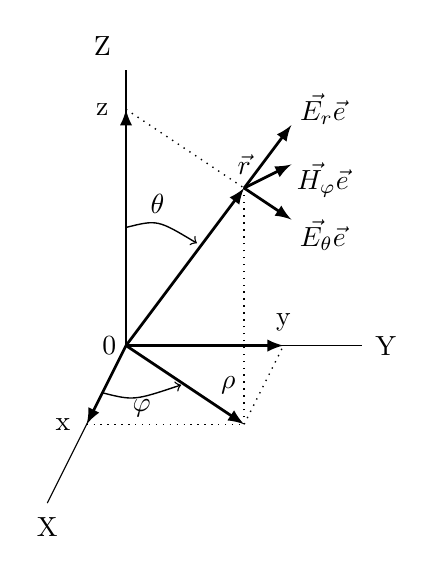
\begin{tikzpicture}
	\draw (4,4) -- (3,2)node at (3, 1.7) {X};%Fadenkreuz x
	\draw (4,4) node[left] {0} -- (7,4)node at (7.3, 4) {Y};%Fadenkreuz y
	\draw (4,4) -- (4,7.5)node at (3.7, 7.8) {Z};%Fadenkreuz z
	
	\draw[line width=1pt, ->, >=latex](4, 4)  -- (3.5, 3) node at (3.2, 3) {x};
	\draw[line width=1pt, ->, >=latex](4, 4)  -- (6, 4) node at (6, 4.3) {y};
	\draw[line width=1pt, ->, >=latex](4, 4)  -- (4, 7) node at (3.7, 7) {z};
	
	\draw[line width=0.5pt, style=dotted](3.5, 3) -- (5.5, 3);%Projektion y Rcihtung
	\draw[line width=0.5pt, style=dotted](5.5, 3) -- (6, 4);%Projektion x Rcihtung
	
	\draw[line width=1pt, ->, >=latex](4, 4)  -- (5.5, 3) node at (5.3, 3.5) {$\rho$};
	
	\draw[line width=1pt, ->, >=latex](4, 4)  -- (5.5, 6) node at (5.5, 6.3) {$\vec{r}$};
	
	\draw[line width=0.5pt, style=dotted](5.5, 3) -- (5.5, 6);%Projektion p zu \vec{r}
	\draw[line width=0.5pt, style=dotted](4, 7) -- (5.5, 6);%Projektion von z zur \vec{r}
	
	\coordinate (A) at (4, 5.5);
	\coordinate (B) at (4.9, 5.3);
	\coordinate (a) at (4.4, 5.6);
	\draw[line width=0.5pt, cap=round,->](A) .. controls (a) .. (B) node at (4.4, 5.8){$\theta$};
	
	\coordinate (C) at (3.7, 3.4);
	\coordinate (D) at (4.7, 3.5);
	\coordinate (c) at (4.1, 3.3);
	\draw[line width=0.5pt, cap=round,->](C) .. controls (c) .. (D) node at (4.2, 3.2){$\varphi$};
	
	%Einheitsvektoren
	\draw[line width=1pt, ->, >=latex](5.5, 6)  -- (6.1, 6.8) node at (6.5, 7) {$\vec{E_{r}}\vec{e}$};
	\draw[line width=1pt, ->, >=latex](5.5, 6)  -- (6.1, 5.6) node at (6.5, 5.4) {$\vec{E_{\theta}}\vec{e}$};
	\draw[line width=1pt, ->, >=latex](5.5, 6)  -- (6.1, 6.3) node at (6.5, 6.1) {$\vec{H_{\varphi}}  \vec{e}$};
	
\end{tikzpicture}
\end{center}
	\caption{Feldvektor mit Einheitsvektoren}
	\label{fig:FerdVektorEinheistsvektor}
\end{figure}

Die Oberfläche  der elektromagnetische Welle mimmt mit steigendem Abstand r von der Antenne immer weiter zu. Ebendfals nimmt die Beugung der Oberfläche der Kugelwelle immer mehr ab. Ist der Abstand r genügend gross, so kann die Welle lokal als Ebene Wellenfront angenommen werden. Bei Distanzen von mehr als $2\lambda$ kann das Fernfeld angenommen werden. Bei einer Zielfrequenz von 2.45 Ghz bei der die Bluetooth Antenne arbeiten soll, tritt das Fernfeld wie in der Gleichung \ref{eq:Fernfeld} gezeit nach 24cm auf.



\begin{align}\label{eq:Fernfeld}
\lambda &=\dfrac{c}{f} \\
\lambda &=\dfrac{3E8[m/s]}{2.45E9[1/s]}=0.12m\\ \nonumber
2\lambda &= Fernfeldkriterium\\ \nonumber
2\lambda &= 2*0.12[m] =0.24[m] \nonumber
\end{align}

Es kann kein eindeutiger Betriebsfall für die "Connect 1"\  Geräte genannt werden, aber es ist warscheindlich, dass die meiseten der Tuchflierpiloten, die die "Connect 1"\  Geräte zur Navigation verwenden, das Gerät auf dem Schoss tragen. Dabei wird das Gerät in einer Hülle mit Bänder am Oberschäkel befestig. Ein Mobieltelefon, welches sich am Arm des Poiloten oder in einer Brusttasche befindet, ist klar mehr als $2\lambda$ entfährtn und somit im Fernfeld. Da sowohl die Loop als auch die Dipol Antenne ein Torus ändliches Fernfeld aufzeigen und die Position der neuen Bluetooth Antenne, für beide Antennen die selbe sein wird, sind die Nafeldeigenschaften der Antennen von bedeutung.

\subsection{Dipol Antenne}
Der Dipol Antenne ist eine häufig vorkommende Antennenform.  Wird der Halbwellendipol mit seiner Resonanzfrequenz $f=\dfrac{\lambda}{2}$ angesteuert, tritt maximales Schwingen des Dipols auf.
%%%%%%%%%%%%%%%%%%%%%%%%%%%%%%%%%%%%%%%%%%%%%%%%%%%
\begin{figure}[h]%ESB Antenne
	\begin{center}
	\begin{tikzpicture}
	\draw[line width=1.5pt](5, 2) circle (0.5) node at (5, 2) {AC};
	\draw[line width=1pt, -*](4.8, 2.45) -- (4.8, 3.6);%nach oben links
	\draw[line width=1pt, -*](5.2, 2.45) -- (5.2, 3.6);%nach oben rechts
	
	\draw[line width=3pt](4.8, 3.5) -- (2, 3.5);%links
	\draw[line width=3pt](5.2, 3.5) -- (8, 3.5);%rechts
	
	\draw[line width=1pt, ->, >=latex](3.8, 3.7)  -- (3, 3.7) node at (3.4, 3.9) {I};%Strompfeil links
	\draw[line width=1pt, ->, >=latex](6.2, 3.7)  -- (7, 3.7) node at (6.6, 3.9) {I};%Strompfeil rechts	
	
	\coordinate (A) at (2, 3.5);%Bogen
	\coordinate (B) at (8, 3.5);
	\coordinate (a) at (5, 5.2);
	\draw[line width=1pt, cap=round](A) .. controls (a) .. (B);
	
	\draw[line width=0.5pt, style=densely dashed](1.8, 3.5) -- (1.8, 5.5);%nach oben links
	\draw[line width=0.5pt, style=densely dashed](8.2, 3.5) -- (8.2, 5.5);%nach oben rechts
	\draw[line width=0.5pt, style=densely dashed](1.7, 5.4) -- (8.3, 5.4) node at (5, 5.7) {$\lambda/2$};%langer Strich
	
	\end{tikzpicture}
	\end{center}
\caption{horizontalpolarisierter Halbwellendipol}
\label{fig:HalbWellenDipolHorizontal}
\end{figure}
%%%%%%%%%%%%%%%%%%%%%%%%%%%%%%%%%%%%%%%%%%%%%%%%%%%%%%%%%%%%


Gegenüber idealen Betrachtungen muss die Länge des $\lambda /2$ Dipols um den Faktor 0,95
kürzer gewählt werden, um auf die gewünschte Frequenz zu erhalten, die ist in der Abbildung \ref{fig:HalbWellenDipolHorizontal} gezeigt.
%H. Cuno, Vorbereitung auf die Amateurfunklizenzprüfung, Frech-VerlagStuttgart, 1976 
Ideale Betrachtungen gehen von einem unendlich dünnen Draht aus, wobei der Dipol im
ungestörten Raum betrieben wird. Auf Grund der geforderten mechanischen Festigkeit
müssen reale Dipole eine gewisse Mindestdicke aufweisen. Die Umgebung des Dipols kann
ebenfalls nicht als völlig freier Raum angenommen werden. Es befinden sich immer eine Quelle oder eine Zuleitung oder beides in der Nähe von realen Antennen. Die Dipolenden weisen eine höhere Kapazität als im Idealzustand auf und die Resonanzfrequenz sinkt. Wenn sich eine $\lambda /2$ lange Vertikalantenne über Erde befindet, die vertikal ausgerichtet ist, ergeben sich für das Strahlungsdiagramm die folgenden Eigenschaften: 
Die Horizontalcharakteristik des vertikalen Halbwellendipols ist kreisförmig auf Grund der Symmetrie (das Strahlungsdiagramm ist unabhängig vom Azimutwinkel $\varphi$). Die Vertikalcharakteristik des vertikalen Halbwellendipols über Erde erscheint jedoch gerichtet, das heisst es besteht eine Abhängigkeit vom Winkel $\theta$ . 

Gemäss O. Zinke %O. Zinke, H. Brunswig, Lehrbuch der Hochfrequenztechnik, Band 1, 4. Auflage,Springer-Verlag, Berlin Heidelberg New York, 1990
 lassen sich die folgenden Aussagen für einen Dipol vertikal Polarisiert über der Erde treffen:


\begin{equation}\label{eq:FDipolTheat}
F(\theta,\frac{l}{\lambda}=\dfrac{1}{2})=\dfrac{2\cos^{2}(\dfrac{\pi}{2}\cos\theta)}{\cos\theta}
\end{equation}


Die Nahfeldeigenschaften der Dipol Antenne zeigt ein starkes E Feld. Dieses zeigt eine Richtungsabhänigkeit in Abhänigkeit des Winkels $\theta$. Die Starken E Felder polarisieren alle Dielektrika in unmittelbarer Nähe des Dipols. Dies Führt zu Dielektrischenverlusten. Diese steigen mit der Frequenz des Feldes. Die Dielektrischen Verluste können als Widerstände in serie gedacht werden. Sie stellen die equivaltene Verlustleistung an einem Widerstand dar, die für das Polarisieren der Dielektrikumstruktur nötig ist.
Das Dielektrikum ist eine elektisch nicht leitendes Material, dass aber vom Elektischen Feld durchdingt wird. Die Feldgrössen des Dielektrikums sind die elektrische Feldstärke E und die elektrische Flussdichte D, welche im elektrostatischen Fall, das heisst im zeitlich konstanten Fall, und in einem isotropen Medium durch die Permittivität $\varepsilon $ \ über folgende Beziehung in Gleichung \ref{eq:FlussdichteD} verknüpft sind:


\begin{equation}\label{eq:FlussdichteD}
D=\varepsilon E
\end{equation}

Die Permittivität $\varepsilon$ setzt sich, wie in Gleichung\ref{eq:Epsilon} gezeigt, aus der elektrischen Feldkonstante $\varepsilon_0$ und der materialspezifischen relativen Permittivität $\varepsilon_r$ zusammen:
\begin{equation}\label{eq:Epsilon}
\varepsilon = \varepsilon_r \varepsilon_0
\end{equation}

Da in einem Dielektrikum die Ladungsträger nicht frei beweglich sind, werden sie durch ein äusseres elektrisches Feld polarisiert. Dabei wird zwischen zwei Arten der Polarisation unterschieden:
\begin{itemize}
\item Verschiebungspolarisation
\item Orientierungspolarisation
\end{itemize}
Bei der Verschiebungspolarisation werden elektrische Dipole  induziert, das heisst Dipole entstehen durch geringe Ladungsverschiebung in den Atomen oder Molekülen oder zwischen verschieden geladenen Ionen. Bei einem Wechselfeld „schwingen“ die negative Elektronenhülle und der positive Atomkern gegenläufig hin und her. Die bei diesen Schwingungen entsteht  Wärmeenergie kann gegenüber der Enegie die bei der Orientierungspolarisation vernachlässigt werden.  Denn die Bewegung des Atomkerns kann auf Grund seiner deutlich grösseren Masse  gegenüber der Elektronenhüllenbewegung vernachlässigt werden. Somit wird der Atomkern als ortsfest betrachtet. 

Unter der Orientierungspolarisation versteht man die Ausrichtung ungeordneter, permanenter Dipole eines Isolators im elektrischen Feld gegen ihre thermische Bewegung. Bei einem Wechselfeld müssen sich die Moleküle ständig umorientieren, wodurch Wärmeenergie entsteht.

Im Nahfeld einer Antenne pendelt die nicht abgestrahlte Energie im Raum um die Antenne hin un der. Das Nahfeld baut sich auf und wider ab und wechselt so mit der Resonanzrequenz $f$ seine Richtung. Werden die Moleküle im Dielektischen Raum um die Antenne bei jeder Schwinung neu polarisiert, also bei jeder Schwinung neu Ausgerichtet.
Die im Dielektrikum gespeicherte Energie ist stark von der materialspezifischen relativen Permittivität $\varepsilon_r $ abhänig. 

\subsection{Loop Antenne}
Magnetische Antennen sprechen nur auf die magnetischen Feldlinien des elektromagnetischen Feldes an, weshalb sie magnetische Antennen genannt werden. Sie sind nicht, wie oft angenommen wird, magnetisch. Nur in unmittelbarer Nähe der Antenne ist ein starkes magnetisches Feld vorhanden, und bereits nach $\lambda/4$ Wellenlänge ist ein starkes elektrisches Feld vorhanden. Die magnetischen Feldlinien treten bei magnetischen Antennen senkrecht durch die Loop-Fläche hindurch. Für maximalen Empfang muss deshalb die Schmalseite der magnetischen Antenne in Richtung des Senders

\subsection{Eigenschaften der Antenne}\label{sec:EigenschaftenAntenne}
Die 2.4 GHz Bluetooth Antenne wird im Gerät "Connect 1" der Flytec eingesetz. Dies ist ein kommpaktes Gandgerät welches den Piloten eines Tuchfliegers bei der Navigation in der Luft unterstütz. Die Geräteabmessungen sind 142 x 88 x 23 mm (L x B x H). Der Raum der die neue Antenne einnehem wird ist nicht der Selbe wie im der Vorgängerversion der "Connect 1" Hardware. Für die neue positionierung der Antenne wird der Hohlraum zwischn der Seitenwand des ABS Kunsstoffgehäuse und der Hauptplatinen befestigungsleiste im Inneren des "Connect 1" vorgesehen. Das mögliche Antennenvolumen beschränkt sich somit auf 55 x 10 x 3.5 mm (L x B x H).\\
Die Speisung der neuen Bluetooth Antenne soll nicht wie bis anhin asymmetisch sein. Wie der Antennenfusspunkt mit der Quelle verbunden wird ist zum jetzigen Zeitpunkt noch nicht definiert. Mögliche symmetrische Verbindungen sind:
\begin{itemize}
\item Microstrip Verbindung  
\item Zweidrahtleitung
\item Zweidrahtleitung in Form eines Koaxialkabels
\end{itemize}

Die symmetische Verbindung zwischen Quelle und Antenne hat den Vorteil, dass die bis anhin verwendeten Baluns für die Umwandulung des symmetrischen Ausgangs des Transsivers nicht mehr benötigt werden. \\
Die Ausgangsimpedanz des verwendeteten Texas Instruments CC2541 Transsivers ist bei 2.440 GHz $(70+j30) Ohm$. Dies entspricht einer komplexen Ausgagnsimpedanz. \\Bei den gemachten Aussgagen zu den Simulationen wurde jedoch eine rein reele Quellimpedanz von $(50+j0) Ohm$ angenommen.

\subsection{Halbwellen Dipol Eigenschaften}
Das Erstzschaltbild in der Abbildung \ref{fig:ESBantenne} einer Antenne, zeigt die wesentlichen Parameter, die für eine beurteilung der Abstrahleffizienz verantworlich sind. Es sind dies:
\begin{itemize}
\item $R_{v}$
\item $R_{rad}$
\item $Z_{ant}$
\end{itemize}

%%%%%%%%%%%%%%%%%%%%%%%%%%%%%%%%%%%%%%%%%%%%%%%%%%%
\begin{figure}%ESB Antenne
	\begin{center}
	\begin{tikzpicture}
%	\draw[line width=1.5pt](7, 1.5) rectangle (12, 5.5) node at (9.5, 6) {Anpassungsnetzwerk};
	\draw[line width=1.5pt, *-](12, 5)  -- (13.5, 5);
	\draw[line width=1.5pt, *-](12, 2)  -- (16, 2);
	\draw[line width=1.5pt](13.5, 4.75) rectangle (14.5, 5.25) node at (14, 5.5) {$R_{v}$};
	\draw[line width=1.5pt](14.5, 5)  -- (16, 5);
	\draw[line width=1.5pt](16, 5)  -- (16, 4.4);
	\draw[line width=1.5pt](15.75, 3.4) rectangle (16.25, 4.4) node at (17, 3.9) {$R_{rad}$};%Rrad
	\draw[line width=1.5pt](16, 3.4)  -- (16, 2.8);
	\draw[line width=1.5pt](15.75, 2.8)  -- (16.25, 2.8);%Kondensator oben
	\draw[line width=1.5pt](15.75, 2.6)  -- (16.25, 2.6);%Kondensator unten
	\node at (17, 2.7) {$X_{ant}$};
	\draw[line width=1.5pt](16, 2.6)  -- (16, 2);
	
%	\draw[line width=1.5pt, ->, >=latex](6.5, 4)  -- (8, 4) node at (8, 3.5) {$P_{ein}$};
	\draw[line width=1.5pt, ->, >=latex](11.5, 4)  -- (13, 4) node at (13, 3.5) {$P_{ant}$};
	

	\draw [-latex,line width=1.5pt](11.5,1) |-(13,2.5) node at (11.5, 0.5) {$Z_{ant}$};
	
	\node at (17.5, 6) {$\eta_{rad}=\dfrac{R_{rad}}{Rv+R_{rad}}$};
%	\node at (9.5, 7) {$\eta_{overall}=\dfrac{P_{rad}}{P_{ein}}$};
	
	\node at (18, 2.7) {$\varepsilon$};
	\node at (18.5, 2.7) {$\delta$};
	
	\draw[->,line width=0.5pt,decorate, decoration=snake ](18, 4.1) -- (19.5, 4.6);
	\draw[->,line width=0.5pt, decorate, decoration=snake](18, 3.9) -- (19.5, 3.9);
	\draw[->,line width=0.5pt, decorate, decoration=snake](18, 3.7) -- (19.5, 3.1);
	\node at (20, 3.9) {$P_{rad}$};
	\end{tikzpicture}
	\end{center}
\caption{Ersatzschaltbild einer Antenne}
\label{fig:ESBantenne}
\end{figure}
%%%%%%%%%%%%%%%%%%%%%%%%%%%%%%%%%%%%%%%%%%%%%%%%%%%%%%%%%%%%

Der $R_{v}$ vereint die elektrischen Verluste die in den Leitern und an den Übergeängen zu standekommen. Ebensvals kann der $R_{rad}$ nicht einfach ausgemessen werden, $R_{rad}$ entspricht dem Widersand der benötigt würde, um beim frequenzabhänig resultierenden Antennestrom die abgestrhlte Leistung umzuwandeln.\\
Das Verhältnis von $R_{rad}$  zu $R_{v}$ wirk direk in die Abstrahleffizienz $\eta_{rad}$. \\
Die Antennen impedanz ist in der Abbildung \ref{fig:ESBantenne} als $X_{ant}$ in Form eines Kondensator abgebildet. Die Dielektrischenverluste des Winkels $\delta$ wirken ebenfals in den $R_{v}$.\\
Die drei Komponenten $R_{v}$, $R_{rad}$ und $X_{ant}$ ergeben zusammen die gesammte Antennenimpedanz $Z_{ant}$.


Der Halbwellend Dipol der Gleigung \ref{eq:Rrrad} im Kapitel \ref{sec:kurzerDipol}berechnet werden. Man erhält für $2L = \frac{\lambda}{2}$ einen $R_{rad}$ von $15.7 \Omega $.

\subsection{Halbwellen Loop Eigenschaften}
Der Loop als Strahlendes Element besitzt das selbe Ersatzschaltbild wie ein Dipol. Seine strahlenden Eigenschaften sind jedoch nicht die gleichen wie beim Dipol. Der Straluungswiderstand $R_{rad}$ kann mit der Formel \ref{eq:RradLoop} aus Kapitel \ref{sec:LoopAntenneTheorie} berechnet werden. Für einen Loop Antenne der Länge $l=\frac{\lambda}{2}$ findet man $R_{rad} = 12.3\Omega$. Für einen Loop der Länge $l=\frac{\lambda}{2}$ kann mit der Gleichung \ref{eq:XantLoop} einen Wert für $X = 637 \Omega$ gefunden werden. Um X zu berechnen wurde einen Loop Radius a von 1cm und als Leiterduchmesser 0.5mm verwendet. Das Fürhrt zu einen Kreisumfang von $U=D\pi=2a\pi=\lambda /2$. Als Permeabilität $\mu $ für Kupfer wurde der Wert $1.256E^{-10}$ verwendet.
\begin{equation}\label{eq:XantLoop}
X= 2\pi f a(ln \left( \frac{8a}{p} \right) - 1.75)
\end{equation}

Aufgrund der engen Platzverhältnisse, die für das Antennenvolumen herschen, kann keine runde Loop Antenne umgesetzt werden. \\
Die Formgebung muss in dem freien Volumen, welches im Kapitel \ref{sec:EigenschaftenAntenne} beschrieben wurde, platzfinden. Dies führt zu einem langen flachen Loop. Die Form erinnert stark an jehene eines Faltdipols. Die Abbildung \ref{fig:FflacheLoopAntenne} zeigt einen Loop Antenne die, das freie Volumen zwischen der Elektronik des Gerät und der Seitenwand nutzt.\\
 Ein gefalteter Dipol hat in etwa des selbe Abstrahlverhalten wie ein Halbwellen Dipol. Derstrahlungswiderstand ist beinahe vier mal so gross und beträg um die 280 Ohm. 
\begin{figure}[h]
	\begin{center}
	\begin{tikzpicture}
	\draw[line width=1.5pt](3, 3)  -- (3, 4);%links
	\draw[line width=1.5pt](3, 4)  -- (8.5, 4);%oben lang
	\draw[line width=1.5pt](3, 3)  -- (5.5, 3);%unten von links
	\draw[line width=1.5pt](6, 3)  -- (8.5, 3);%unten von rechts
	\draw[line width=1.5pt](8.5, 3)  -- (8.5, 4);%rechts
	%\draw[line width=1.5pt, *-](3, 3)  -- (3, 4);%Speisung
	\draw[line width=1.5pt,*-](5.5, 2.5)  -- (5.5, 3);%Speisung vertikal links
	\draw[line width=1.5pt,*-](6, 2.5)  -- (6, 3);%Speisung vertikal rechts

	\node at (5.75, 2) {Speisung};
	\end{tikzpicture}
	\end{center}
\caption{Flach gestauchte Loop Antenne}
\label{fig:FflacheLoopAntenne}
\end{figure}
\subsection{Vollwellen Loop Eigenschaften}
\subsection{Nutzwertanalyse Antennen Eigenschaften  }
\begin{table}[htb]
  \centering
  \begin{tabular}{l r l l l l l l l l} \toprule 
  && \multicolumn{2}{c}{Dipol $\lambda/2$}   && \multicolumn{2}{c}{Loop $\lambda/2$}   && \multicolumn{2}{c}{Loop} \\ \cmidrule{3-4} \cmidrule{6-7} \cmidrule{9-10}
  Kriterium                  & $g$ \%  & $N$ & $N\cdot g$               && $N$ & $N\cdot g$                  && $N$ & $N\cdot g$ \\ \midrule
  Antennengüte Q            &  25             & 2   & 0.5               && 5   & 1.25                        && 5   & 1.25 \\
  Impedanz                  &  15             & 3   & 0.45              && 4   & 0.6                         && 5   & 0.75 \\
  vvvv    &  20             & 1   & 0.2               && 4   & 0.8                         && 5   & 1 \\
  Richtcharakteristik       &  20             & 1   & 0.2               && 6   & 1.2                         && 6   & 1.2 \\
  Relative Bandbreite       &   5             & 3   & 0.15              && 6   & 0.3                         && 5   & 0.25 \\
  Materialaufwand           &   5             & 6   & 0.3               && 4   & 0.2                         && 6   & 0.3 \\
  Kosten                    &  10             & 4   & 0.4               && 6   & 1.2                         && 6   & 1 \\
  Gesamt                    & 100             &     & 2.2               &&     & 5.55                        &&     & 5.75 \\ \bottomrule
  \end{tabular}
  \caption{Nutzwertanalyse für symmetrische Antenne}
  \label{nutzwertEvaluation}
\end{table}

